\documentclass[
	classe=$2^{de}$,
	exercices=Chapitre\space 2
]{exercice}

\title{Inéquations et intervalles}
\author{}
\date{}

\begin{document}

\maketitle

\begin{enumerate}
	\item Résoudre l'inéquation $3x + 2 ≤ 5$ :

	      \ifdefined\makeCorrection
		      {\color{red}\begin{align*}
				      3x + 2 & ≤ 5 \\
				      3x     & ≤ 3 \\
				      x      & ≤ 1
			      \end{align*}}
	      \else
		      \vspace{8em}
	      \fi

	      On appelera cette inéquation \uline{l'inéquation (A)}.
	\item Résoudre l'inéquation $2x + 2 ≤ 6x + 10$ :

	      \ifdefined\makeCorrection
		      {\color{red}\begin{align*}
				      2x + 2 & ≤ 6x + 10 \\
				      -4x    & ≤ 8       \\
				      x      & ≥ -2
			      \end{align*}}
	      \else
		      \vspace{8em}
	      \fi

	      On appelera cette inéquation \uline{l'inéquation (B)}.
	\item Sur la droite ci-dessous, marquer en {\color{red}rouge} les abscisses qui sont solutions de l'équation (A).
	      \begin{center}
		      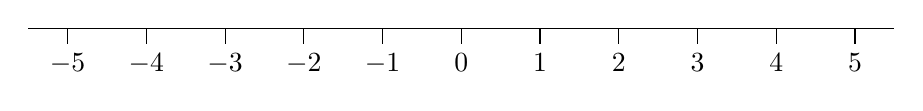
\begin{tikzpicture}
			      \draw[\myArrow] (-5.5,0) -- (5.5,0);
			      \foreach \x in {-5,...,5} {
					      \draw (\x,0) -- ++(0,-0.2) node[below] {$\x$};
				      }
			      \ifdefined\makeCorrection
				      \draw[very thick,red] (-5.5,0) -- (1,0);
			      \fi
		      \end{tikzpicture}
	      \end{center}
	\item Sur la droite ci-dessous, marquer en {\color{blue}bleu} les abscisses qui sont solutions de l'équation (B).
	      \begin{center}
		      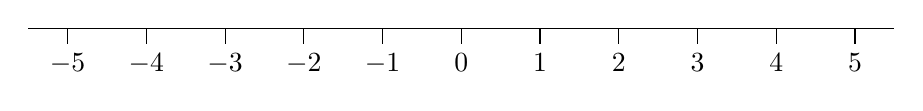
\begin{tikzpicture}
			      \draw[\myArrow] (-5.5,0) -- (5.5,0);
			      \foreach \x in {-5,...,5} {
					      \draw (\x,0) -- ++(0,-0.2) node[below] {$\x$};
				      }
			      \ifdefined\makeCorrection
				      \draw[very thick,blue] (-2,0) -- (5.5,0);
			      \fi
		      \end{tikzpicture}
	      \end{center}
	\item Sur la droite ci-dessous, marquer en {\color{green}vert} les abscisses qui sont solutions de l'équation (A) ET solutions de l'équation (B).
	      \begin{center}
		      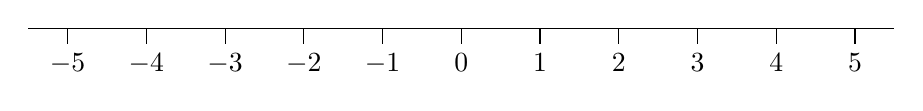
\begin{tikzpicture}
			      \draw[\myArrow] (-5.5,0) -- (5.5,0);
			      \foreach \x in {-5,...,5} {
					      \draw (\x,0) -- ++(0,-0.2) node[below] {$\x$};
				      }
			      \ifdefined\makeCorrection
				      \draw[very thick,green] (-2,0) -- (1,0);
			      \fi
		      \end{tikzpicture}
	      \end{center}
	\item
	      \begin{itemize}
		      \item Comment note-t'on l'ensemble des points {\color{red}rouges} ? \correctionDots{$[-∞ ; 1]$}
		      \item  Comment note-t'on l'ensemble des points {\color{blue}bleus} ? \correctionDots{$[-2 ; +∞]$}
		      \item  Comment note-t'on l'ensemble des points {\color{green}verts} ? \correctionDots{$[-2 ; 1]$}
	      \end{itemize}
\end{enumerate}

\end{document}